\section{Appendix: Properties of the Benchmark and Missing Plots}

\begin{figure*}[h]
\begin{center}
$$ 
\begin{bmatrix}
\frac{1}{2} & -\frac{1}{2} & \frac{1}{2} & -\frac{1}{2} & \frac{1}{2} & -\frac{1}{2}  \\
-\frac{1}{2} & \frac{1}{2} & \frac{1}{2} & -\frac{1}{2} & \frac{1}{2} & -\frac{1}{2} \\
\frac{1}{2} & -\frac{1}{2} & -\frac{1}{2} & \frac{1}{2} & \frac{1}{2} & -\frac{1}{2}  \\
-\frac{1}{2} & \frac{1}{2} & -\frac{1}{2} & \frac{1}{2} & \frac{1}{2} & -\frac{1}{2} \\
\frac{1}{2} & -\frac{1}{2} & \frac{1}{2} & -\frac{1}{2} & -\frac{1}{2} & \frac{1}{2}  \\
-\frac{1}{2} & \frac{1}{2} & \frac{1}{2} & -\frac{1}{2} & -\frac{1}{2} & \frac{1}{2}  \\
\frac{1}{2} & -\frac{1}{2} & -\frac{1}{2} & \frac{1}{2} &-\frac{1}{2} & \frac{1}{2} \\
-\frac{1}{2} & \frac{1}{2} & -\frac{1}{2} & \frac{1}{2}  & -\frac{1}{2} & \frac{1}{2} \\
\end{bmatrix} ~~~~~~~~
% \begin{bmatrix}
% \frac{2}{3} & -\frac{1}{3} & -\frac{1}{3} & \frac{2}{3} & -\frac{1}{3} & -\frac{1}{3}\\
% \frac{2}{3} & -\frac{1}{3} & -\frac{1}{3} & -\frac{1}{3} & \frac{2}{3} & -\frac{1}{3}\\
% \frac{2}{3} & -\frac{1}{3} & -\frac{1}{3} & -\frac{1}{3} & -\frac{1}{3} & \frac{2}{3}\\
%  -\frac{1}{3} & \frac{2}{3} & -\frac{1}{3} & \frac{2}{3} & -\frac{1}{3} & -\frac{1}{3}\\
% -\frac{1}{3} & \frac{2}{3} & -\frac{1}{3} & -\frac{1}{3} & \frac{2}{3} & -\frac{1}{3}\\
% -\frac{1}{3} & \frac{2}{3} &  -\frac{1}{3} & -\frac{1}{3} & -\frac{1}{3} & \frac{2}{3}\\
% -\frac{1}{3} & -\frac{1}{3} & \frac{2}{3} & \frac{2}{3} & -\frac{1}{3} & -\frac{1}{3}\\
% -\frac{1}{3} & -\frac{1}{3} & \frac{2}{3} & -\frac{1}{3} & \frac{2}{3} & -\frac{1}{3}\\
% -\frac{1}{3} & -\frac{1}{3} & \frac{2}{3} & -\frac{1}{3} & -\frac{1}{3} & \frac{2}{3}\\
% \end{bmatrix} 
\begin{bmatrix}
 \frac{2}{3}   & -\frac{1}{3}  & -\frac{1}{3} & \frac{2}{3}   & -\frac{1}{3}  & -\frac{1}{3}   \\
 -\frac{1}{3}  & \frac{2}{3}   & -\frac{1}{3} & \frac{2}{3}   & -\frac{1}{3}  & -\frac{1}{3}   \\
 -\frac{1}{3}  & -\frac{1}{3}  & \frac{2}{3}  & \frac{2}{3}   & -\frac{1}{3}  & -\frac{1}{3}   \\
 \frac{2}{3}   & -\frac{1}{3}  & -\frac{1}{3} & -\frac{1}{3}  & \frac{2}{3}   & -\frac{1}{3}   \\
 -\frac{1}{3}  & \frac{2}{3}   & -\frac{1}{3} & -\frac{1}{3}  & \frac{2}{3}   & -\frac{1}{3}   \\
 -\frac{1}{3}  & -\frac{1}{3}  & \frac{2}{3}  & -\frac{1}{3}  & \frac{2}{3}   &  -\frac{1}{3}  \\
 \frac{2}{3}   & -\frac{1}{3}  & -\frac{1}{3} & -\frac{1}{3}  & -\frac{1}{3}  & \frac{2}{3}    \\
 -\frac{1}{3}  & \frac{2}{3}   & -\frac{1}{3} & -\frac{1}{3}  & -\frac{1}{3}  & \frac{2}{3}    \\
 -\frac{1}{3}  & -\frac{1}{3}  & \frac{2}{3}  & -\frac{1}{3}  & -\frac{1}{3}  & \frac{2}{3}    \\
\end{bmatrix} 
$$
\end{center}
\label{fig1}
\caption{Benchmark construction for $k=2$ and $\alpha=3$ (left) and $k=3$ and $\alpha=2$ (right).}
\end{figure*}


\begin{fact}
For $a\neq a'$, we have $d(\mathcal{C}^{a},\mathcal{C}^{a'}) = 1-1/k$.
\end{fact}
\begin{proof}
Consider an arbitrary vector $v_i^{\ell}$. By construction, the positive entries of $v_i^{\ell}$ range from $k^{\ell-1}\cdot i+1$ to $k^{\ell-1}\cdot (i+1)$. Similarly, the positive entries for the vector $v_j^{\ell-1}$ range from range from $k^{\ell-2}\cdot j+1$ to $k^{\ell-2}\cdot (j+1)$. Therefore, concatenating $v_j^{\ell-1}$ $k$ times into a vector $v'$, $v'$ and $v_i^{\ell}$ can share at most one positive coordinate. Inductively, the same holds true for any concatenation of vectors $v_j^{\ell-h}$.
Thus, the two clusters induced by the columns formed by concatenating the vectors $v$ can share only a $1/k$ fraction of the points. Since each cluster consists of exactly $k^{\alpha}/k$ = $k^{\alpha-1}$ points, the confusion matrix $M$ only has entries $\frac{n}{k^2}$ and for any permutation $\pi$, we have $d(\mathcal{C}^{a},\mathcal{C}^{a'}) = 1-1/k$.
\end{proof}

\begin{fact}
\label{fact:cost}
For any $C_j^a$, we have $\cost_{C_j^a}(\{\mu(C_j^a)\}) = (\alpha-1)\cdot k^{\alpha-2}\cdot (k-1)$.
\end{fact}
\begin{proof}
Without loss of generality, we consider $C_1^0$; the proof is analogous for the other choices of $j$ and $a$. We first note that for any point $A_i \in C_1^0$, the coordinates $A_{i,\ell}$ are identical for $\ell <k$. Furthermore for the column $\ell\geq k$, we have by construction $\sum_{A_i\in C_j} A_{i,\ell} = k^{\alpha-1}\cdot \frac{k-1}{k} + (k^{\alpha}-k^{\alpha-1})\frac{1}{k}=k^{\alpha-1}\cdot (\frac{k-1}{k} - (k-1)\frac{1}{k}) = 0.$ Therefore, the mean of $C_1^0$ satisfies $\mu(C_1^0)_{\ell} = \begin{cases}A_{i,\ell} &\text{if }\ell<k \\
0 &\text{else.}\end{cases}$. 
Thus, the cost is precisely $(\alpha-1)\cdot k^{\alpha-1}\cdot \left(\left(\frac{k-1}{k}\right)^2 + \left(\frac{1}{k}\right)^2 \right)=(\alpha-1)\cdot k^{\alpha-2}\cdot (k-1)$.
\end{proof}

Finally, we show that the means for the clustering $\mathcal{C}^{a}$ also induce $\mathcal{C}^{a}$.

\begin{fact}
\label{fact:opt}
For a clustering $\mathcal{C}^{a}$, let $\mu(C_j^{a})$ denote the mean of cluster $C_j^a$. Then every point  is assigned to its closest center. Moreover, every point $A_i$ of $C_j^a$ has equal distance to any center $\mu(C_h^{a})$ with $h\neq j$.
\end{fact}
\begin{proof}
Again, we assume without loss of generality $a=0$.
Let $A_i$ be an arbitrary point of cluster $C_{h}^{a}$ and consider the mean $\mu(C_j^a)_{\ell} = \begin{cases}A_{i,\ell} &\text{if }\ell<k \\
0 &\text{else.}\end{cases}$ of cluster $C_j^a$. By definition, the positive coordinates of $A_i$ are not equal to the positive coordinates of $\mu(C_j^a)$. The only difference in coordinates between the means of $\mu(C_j^a)$ and $\mu(C_h^a)$ are the first $k$ coordinates, as the rest are $0$.
But here the coordinates of $\mu(C_h^a)$ and $A_i$ are identical, hence $\mu(C_j^a)$ cannot be closer to $A_i$.

To prove that the distances between $A_i$ and any $\mu(C_h^{a})$ with $h\neq j$ are equal, again consider that any difference can only exist among the first $k$ coordinates. Here, we have $\mu(C_h^{a})_h = \frac{k-1}{k}$, and the remaining columns are $-\frac{1}{k}$. Since $A_{i,h} = -\frac{1}{k}$ for any $h\neq j$, the claim follows.
\end{proof}



\begin{figure}[ht]
  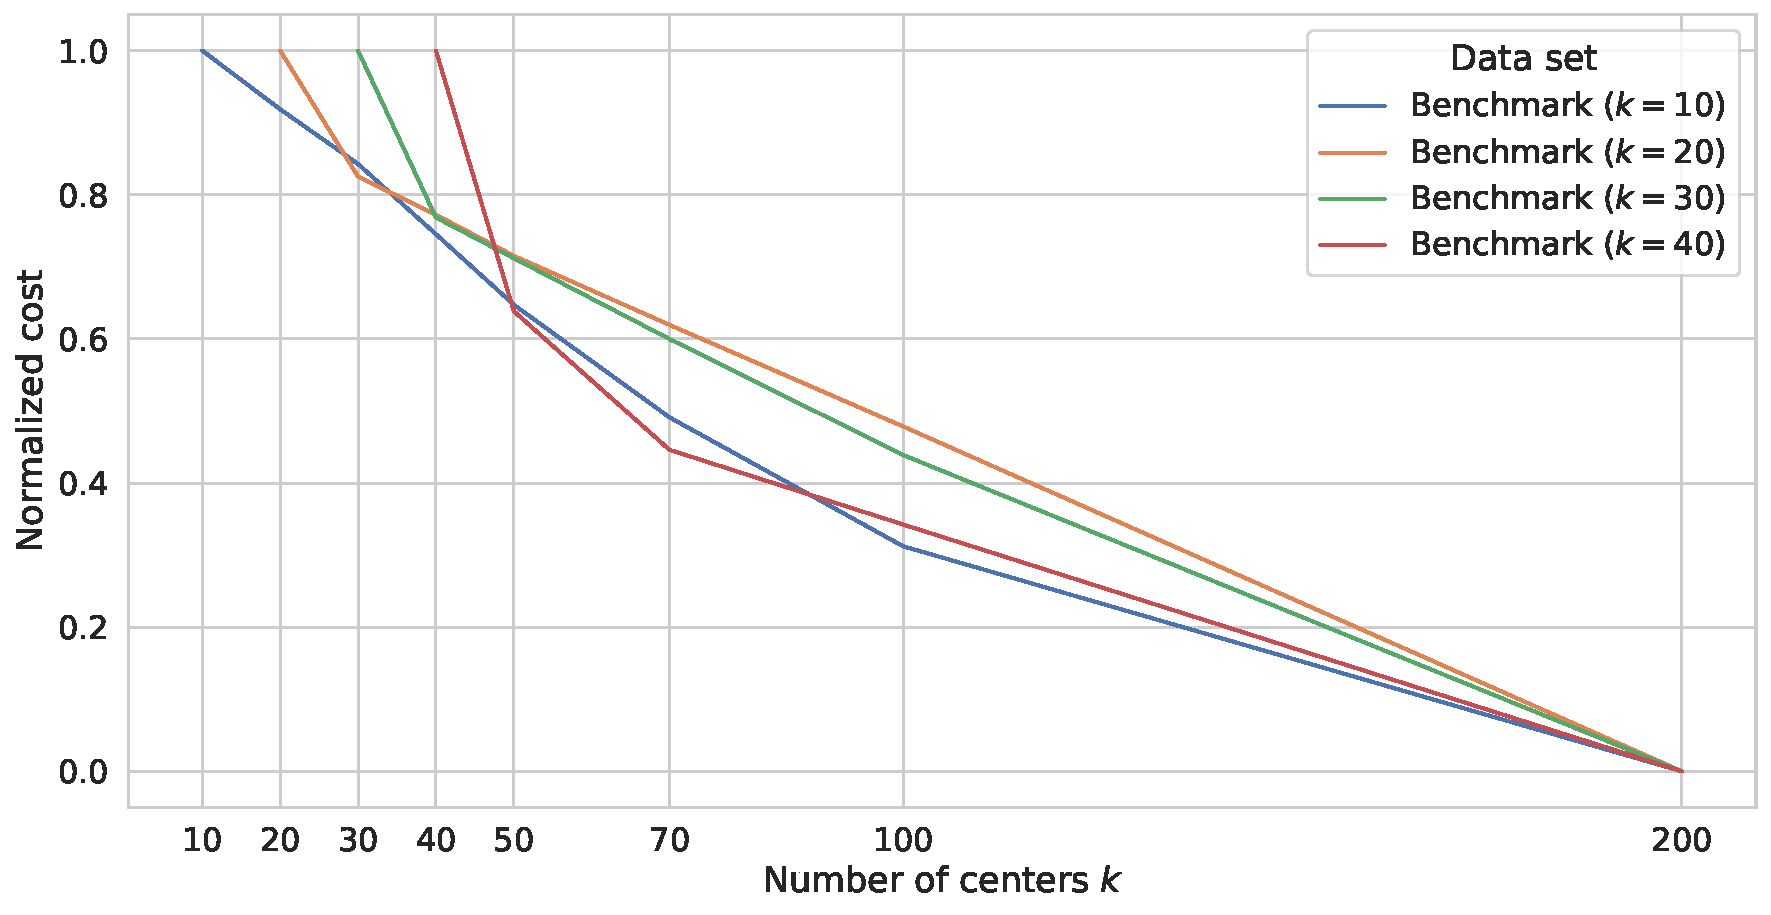
\includegraphics[width=1\linewidth]{figures/cost-curves-benchmark.pdf}
  \caption{Shows the clustering costs of four instances of the benchmark framework as a function of the number of centers. In contrast to real-world data sets, the costs do not decrease rapidly as more cluster centers are added.
  }
  \label{fig:cost-curves-benchmark}
\end{figure}

\begin{figure}[ht]
  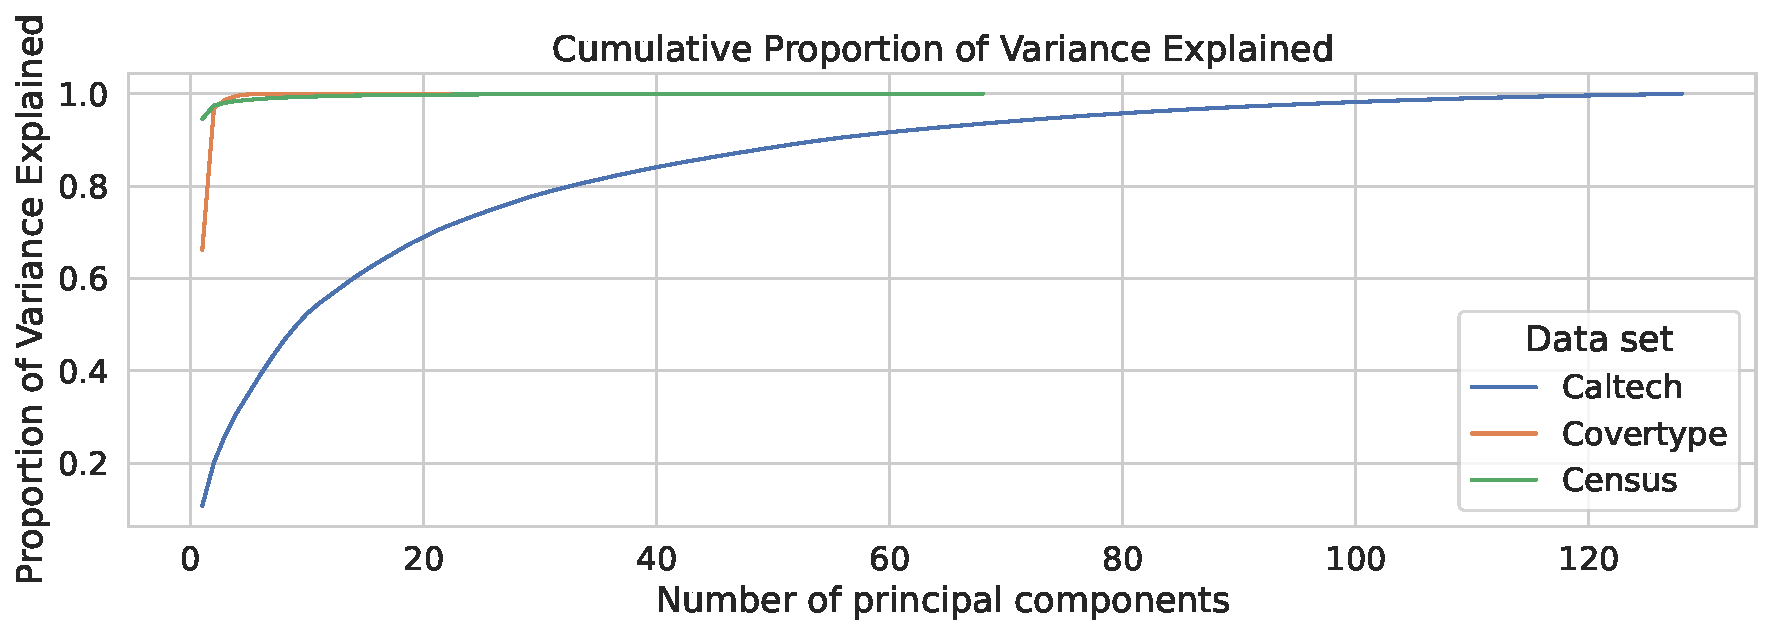
\includegraphics[width=0.9\linewidth]{figures/explained-variance-plot.pdf}
  \caption{The cumulative propotion of explained variance by principal components on \textit{Caltech}, \textit{Covertype}, and \textit{Census}.}
  \label{fig:explained-variance-pca}
\end{figure}


\begin{table}[!htbp]
\centering
\begin{tabular}{lllllll}
\toprule
\parbox[t]{2cm}{\ \\Data set}  & \parbox[t]{5mm}{\ \\$k$} &           BICO & \parbox[t]{1cm}{Group\\Sampling} &      Ray Maker & \parbox[t]{1cm}{Sensitivity\\Sampling} &    StreamKM++ \\
% Dataset & $k$ &                &                &                &                      &               \\
\midrule
Benchmark & 10  &   2.93 (0.144) &   1.01 (0.002) &   3.49 (0.055) &         1.02 (0.003) &  1.04 (0.002) \\
      & 20  &   2.87 (0.137) &   1.01 (0.002) &   3.90 (0.112) &         1.02 (0.003) &  1.11 (0.002) \\
      & 30  &   2.34 (0.070) &   1.02 (0.001) &   4.19 (0.137) &         1.02 (0.002) &  1.10 (0.002) \\
      & 40  &   2.68 (0.230) &   1.02 (0.001) &   3.83 (0.172) &         1.02 (0.002) &  1.17 (0.004) \\
\midrule
Caltech & 10  &   4.15 (0.485) &   1.02 (0.003) &   4.99 (0.124) &         1.01 (0.004) &  1.10 (0.004) \\
      & 20  &   4.16 (0.708) &   1.02 (0.003) &   4.86 (0.134) &         1.01 (0.003) &  1.12 (0.004) \\
      & 30  &   4.15 (0.416) &   1.02 (0.001) &   4.78 (0.117) &         1.01 (0.002) &  1.13 (0.003) \\
      & 40  &   4.18 (0.486) &   1.02 (0.002) &   4.73 (0.068) &         1.01 (0.002) &  1.13 (0.001) \\
      & 50  &   3.99 (0.560) &   1.02 (0.002) &   4.72 (0.090) &         1.01 (0.002) &  1.13 (0.002) \\
\midrule
Census & 10  &   1.65 (0.082) &   1.03 (0.011) &   1.74 (0.044) &         1.02 (0.006) &  1.05 (0.005) \\
      & 20  &   1.74 (0.054) &   1.02 (0.004) &   1.75 (0.038) &         1.01 (0.005) &  1.06 (0.003) \\
      & 30  &   1.77 (0.063) &   1.02 (0.003) &   1.79 (0.032) &         1.01 (0.005) &  1.07 (0.002) \\
      & 40  &   1.83 (0.038) &   1.02 (0.002) &   1.81 (0.021) &         1.01 (0.005) &  1.08 (0.003) \\
      & 50  &   1.87 (0.088) &   1.02 (0.002) &   1.85 (0.044) &         1.01 (0.003) &  1.10 (0.059) \\
\midrule
Covertype & 10  &   1.10 (0.002) &   1.03 (0.011) &   1.18 (0.016) &         1.02 (0.007) &  1.01 (0.002) \\
      & 20  &   1.11 (0.004) &   1.03 (0.010) &   1.21 (0.015) &         1.01 (0.007) &  1.01 (0.002) \\
      & 30  &   1.10 (0.003) &   1.03 (0.005) &   1.22 (0.008) &         1.01 (0.005) &  1.01 (0.002) \\
      & 40  &   1.09 (0.001) &   1.03 (0.005) &   1.22 (0.012) &         1.01 (0.005) &  1.01 (0.001) \\
      & 50  &   1.07 (0.001) &   1.03 (0.003) &   1.22 (0.008) &         1.01 (0.002) &  1.01 (0.001) \\
\midrule
NYTimes & 10  &  18.59 (5.356) &   1.04 (0.003) &  15.37 (0.740) &         1.02 (0.004) &  1.75 (0.105) \\
      & 20  &   9.98 (1.559) &   1.04 (0.003) &  12.71 (0.448) &         1.01 (0.004) &  1.69 (0.024) \\
      & 30  &   8.03 (2.156) &   1.04 (0.002) &  12.18 (0.974) &         1.02 (0.003) &  1.66 (0.030) \\
      & 40  &   6.31 (0.436) &   1.03 (0.003) &  11.20 (0.742) &         1.01 (0.002) &  1.63 (0.024) \\
      & 50  &   5.97 (0.381) &   1.03 (0.002) &  10.81 (0.571) &         1.01 (0.002) &  1.63 (0.026) \\
\midrule
Tower & 20  &   1.07 (0.003) &   1.02 (0.007) &   1.06 (0.004) &         1.03 (0.009) &  1.02 (0.001) \\
      & 40  &   1.06 (0.004) &   1.02 (0.006) &   1.06 (0.002) &         1.02 (0.007) &  1.02 (0.001) \\
      & 60  &   1.06 (0.001) &   1.03 (0.004) &   1.05 (0.004) &         1.01 (0.003) &  1.02 (0.001) \\
      & 80  &   1.05 (0.001) &   1.03 (0.005) &   1.05 (0.002) &         1.01 (0.006) &  1.02 (0.001) \\
      & 100 &   1.04 (0.002) &   1.03 (0.004) &   1.05 (0.001) &         1.01 (0.004) &  1.02 (0.001) \\
\bottomrule
\end{tabular}
\caption{Distortions of the evaluation algorithms on all data sets without PCA preprocessing. Each cell specify the mean distortion along with the standard deviation in brackets of 10 repetition of the experiment.}
\label{tab:distortions-mean-std-without-pca}
\end{table}




\begin{table}[!htbp]
\centering
\begin{tabular}{lllllll}
\toprule
\parbox[t]{2cm}{\ \\Data set}  & \parbox[t]{5mm}{\ \\$k$} &           BICO & \parbox[t]{1cm}{Group\\Sampling} &      Ray Maker & \parbox[t]{1cm}{Sensitivity\\Sampling} &    StreamKM++ \\
\midrule
Caltech+PCA & 10  &   1.16 (0.004) &   1.01 (0.002) &   1.19 (0.009) &         1.00 (0.001) &  1.02 (0.002) \\
      & 20  &   1.42 (0.016) &   1.01 (0.002) &   1.51 (0.008) &         1.01 (0.001) &  1.04 (0.002) \\
      & 30  &   1.73 (0.045) &   1.02 (0.001) &   1.83 (0.014) &         1.01 (0.001) &  1.06 (0.002) \\
      & 40  &   2.13 (0.083) &   1.02 (0.002) &   2.16 (0.016) &         1.01 (0.002) &  1.07 (0.002) \\
      & 50  &   2.38 (0.139) &   1.02 (0.001) &   2.49 (0.017) &         1.01 (0.002) &  1.09 (0.002) \\
\midrule
Census+PCA & 10  &   1.18 (0.012) &   1.01 (0.005) &   1.20 (0.016) &         1.02 (0.009) &  1.01 (0.002) \\
      & 20  &   1.44 (0.046) &   1.02 (0.003) &   1.45 (0.019) &         1.02 (0.010) &  1.04 (0.002) \\
      & 30  &   1.64 (0.044) &   1.02 (0.004) &   1.63 (0.021) &         1.01 (0.007) &  1.06 (0.003) \\
      & 40  &   1.77 (0.035) &   1.02 (0.002) &   1.76 (0.028) &         1.01 (0.004) &  1.07 (0.002) \\
      & 50  &   1.87 (0.068) &   1.02 (0.002) &   1.82 (0.017) &         1.01 (0.004) &  1.08 (0.002) \\
\midrule
Covertype+PCA & 10  &   1.11 (0.003) &   1.03 (0.012) &   1.19 (0.011) &         1.02 (0.010) &  1.02 (0.002) \\
      & 20  &   1.11 (0.003) &   1.03 (0.006) &   1.21 (0.010) &         1.02 (0.007) &  1.02 (0.002) \\
      & 30  &   1.10 (0.002) &   1.03 (0.007) &   1.22 (0.011) &         1.01 (0.005) &  1.01 (0.002) \\
      & 40  &   1.09 (0.002) &   1.03 (0.006) &   1.23 (0.010) &         1.01 (0.005) &  1.01 (0.001) \\
      & 50  &   1.07 (0.001) &   1.03 (0.003) &   1.23 (0.008) &         1.01 (0.003) &  1.01 (0.001) \\
\midrule
NYTimes+PCA & 10  &   1.01 (0.000) &   1.00 (0.000) &   1.01 (0.001) &         1.00 (0.000) &  1.00 (0.000) \\
      & 20  &   1.02 (0.000) &   1.00 (0.000) &   1.02 (0.001) &         1.00 (0.000) &  1.01 (0.000) \\
      & 30  &   1.03 (0.000) &   1.00 (0.000) &   1.03 (0.001) &         1.00 (0.000) &  1.01 (0.000) \\
      & 40  &   1.04 (0.001) &   1.00 (0.000) &   1.04 (0.001) &         1.00 (0.002) &  1.01 (0.000) \\
      & 50  &   1.04 (0.002) &   1.00 (0.000) &   1.05 (0.001) &         1.00 (0.000) &  1.02 (0.000) \\
\bottomrule
\end{tabular}
\caption{Distortions of the evaluation algorithms on the data sets preprocessed with PCA. Each cell specify the mean distortion along with the standard deviation in brackets of 10 repetitions.}
\label{tab:distortions-mean-std-with-pca}
\end{table}



\begin{figure*}
  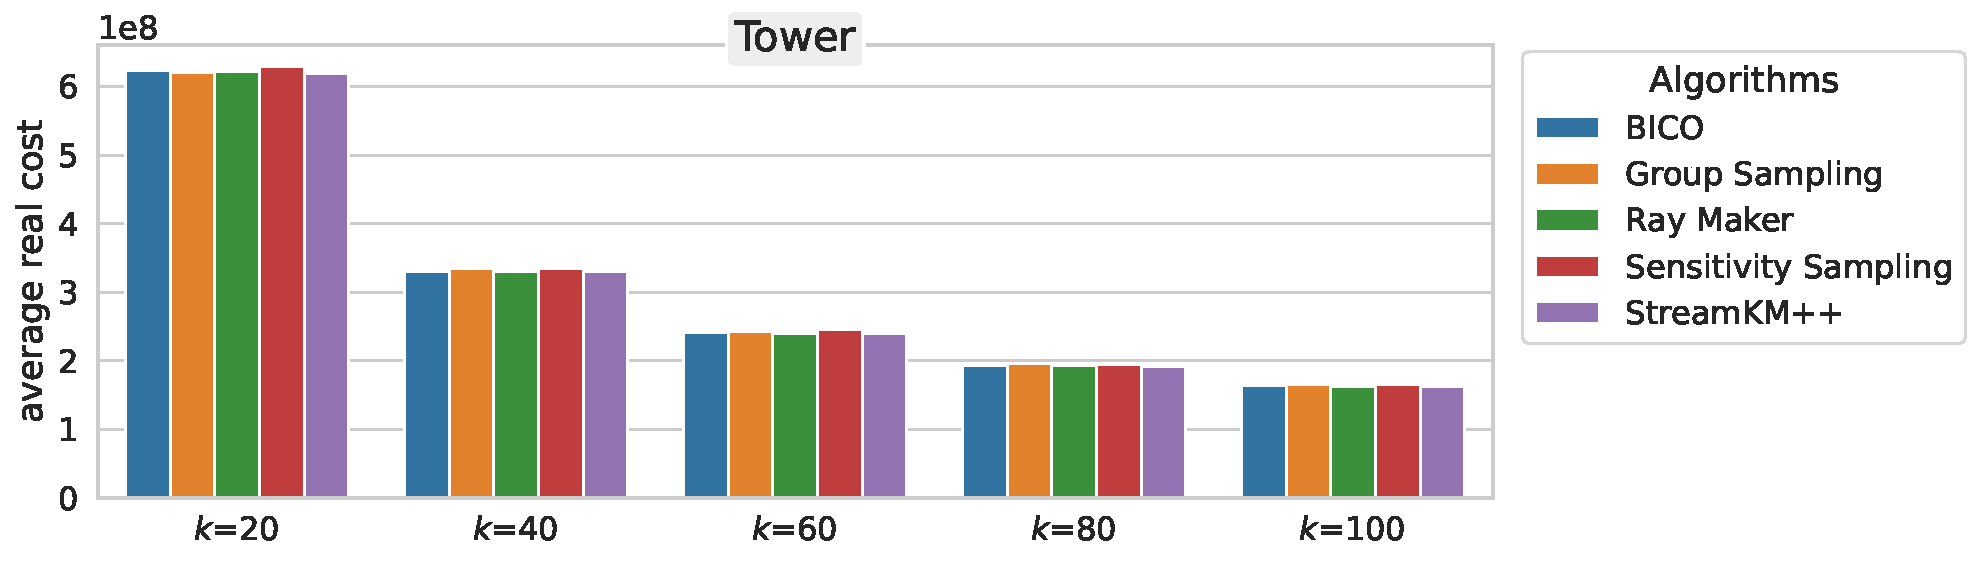
\includegraphics[width=.67\linewidth]{figures/real-costs-Tower.pdf}
  \newline
  \subfloat{
    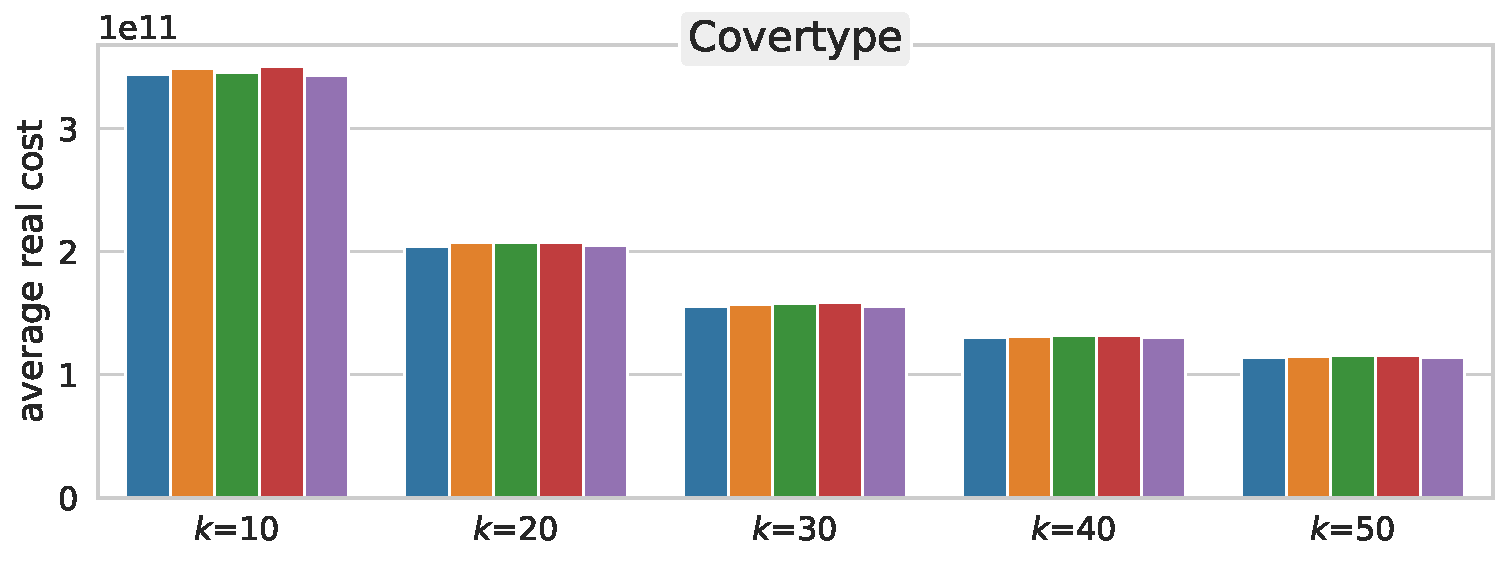
\includegraphics[width=0.5\textwidth]{figures/real-costs-Covertype.pdf}
  }
  \subfloat{
    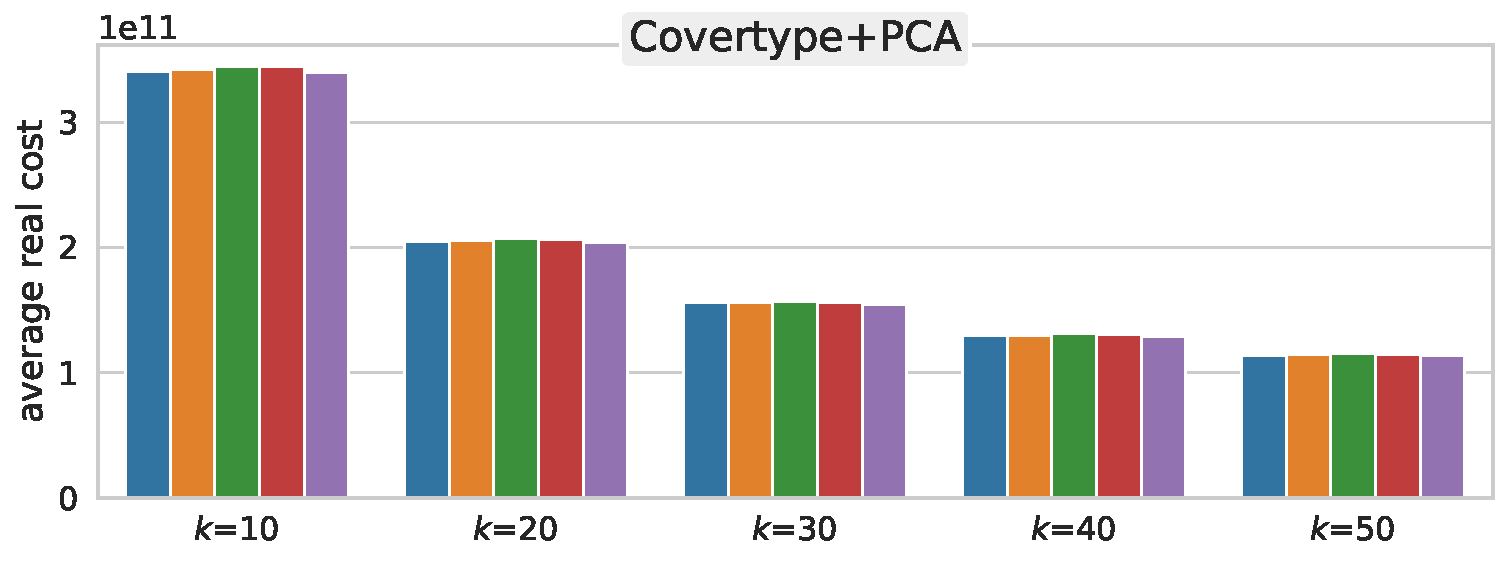
\includegraphics[width=.5\linewidth]{figures/real-costs-Covertype+PCA.pdf}
  }
  \newline\newline
  \subfloat{
    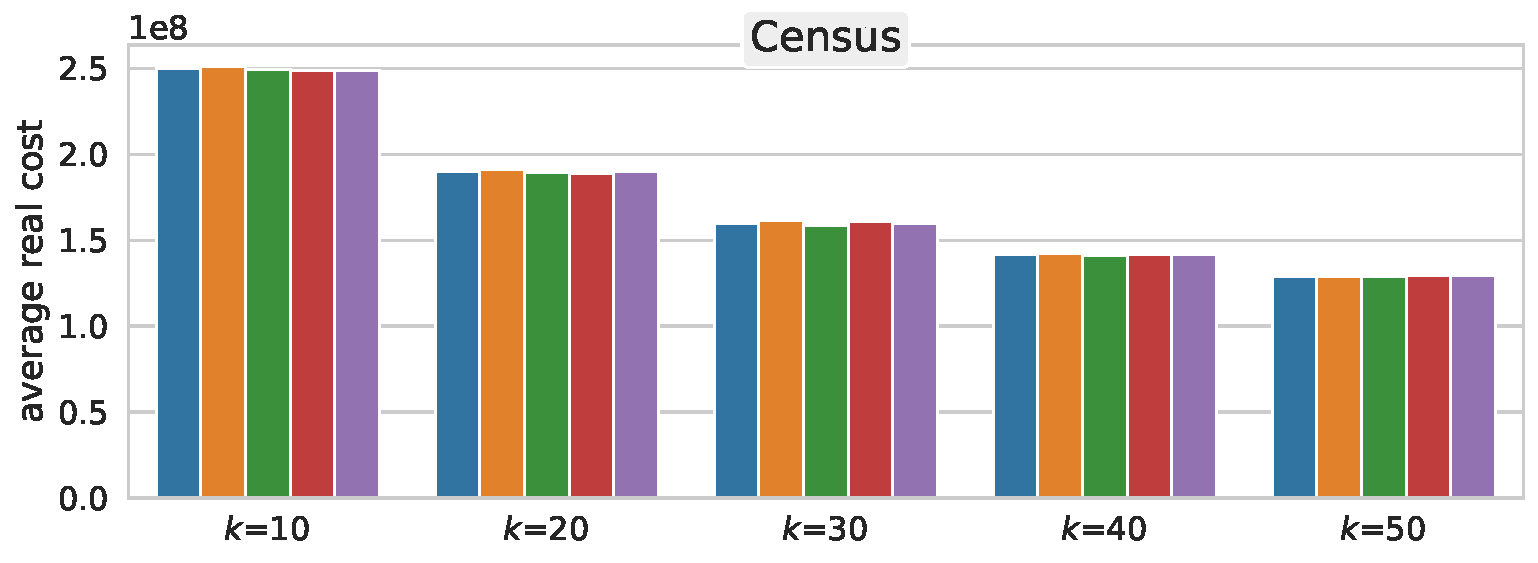
\includegraphics[width=0.5\textwidth]{figures/real-costs-Census.pdf}
  }
  \subfloat{
    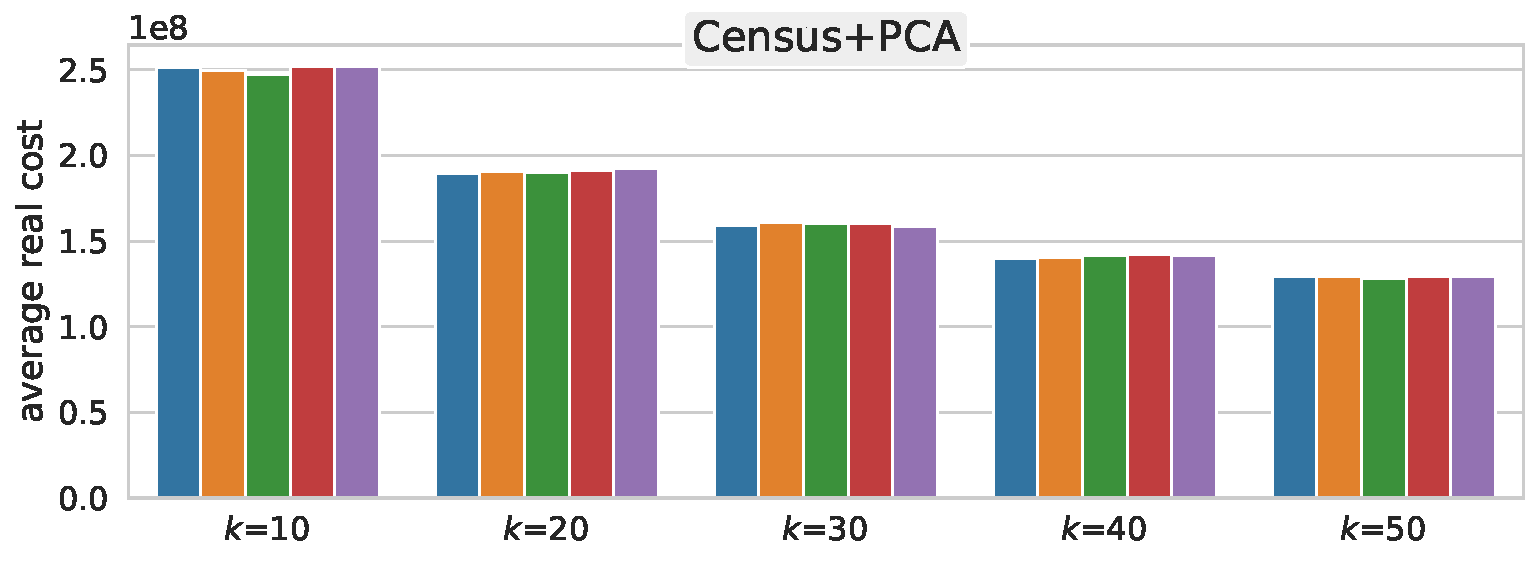
\includegraphics[width=.5\linewidth]{figures/real-costs-Census+PCA.pdf}
  }
  \newline\newline
  \subfloat{
    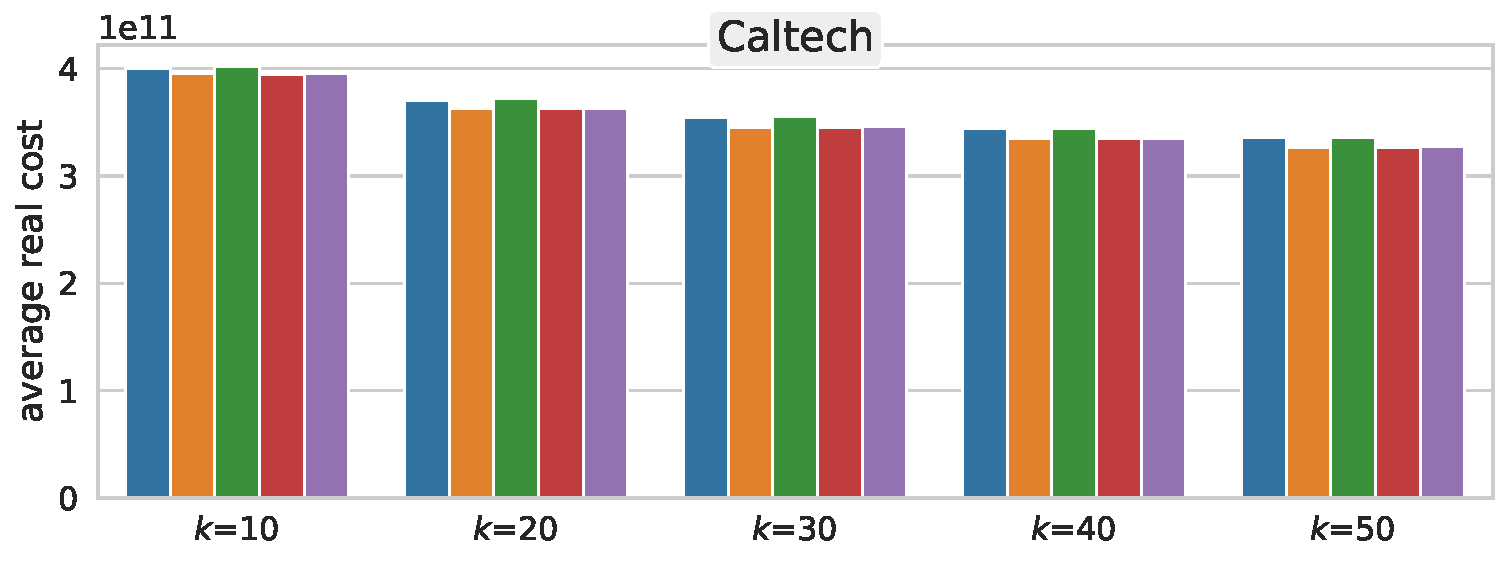
\includegraphics[width=0.5\textwidth]{figures/real-costs-Caltech.pdf}
  }
  \subfloat{
    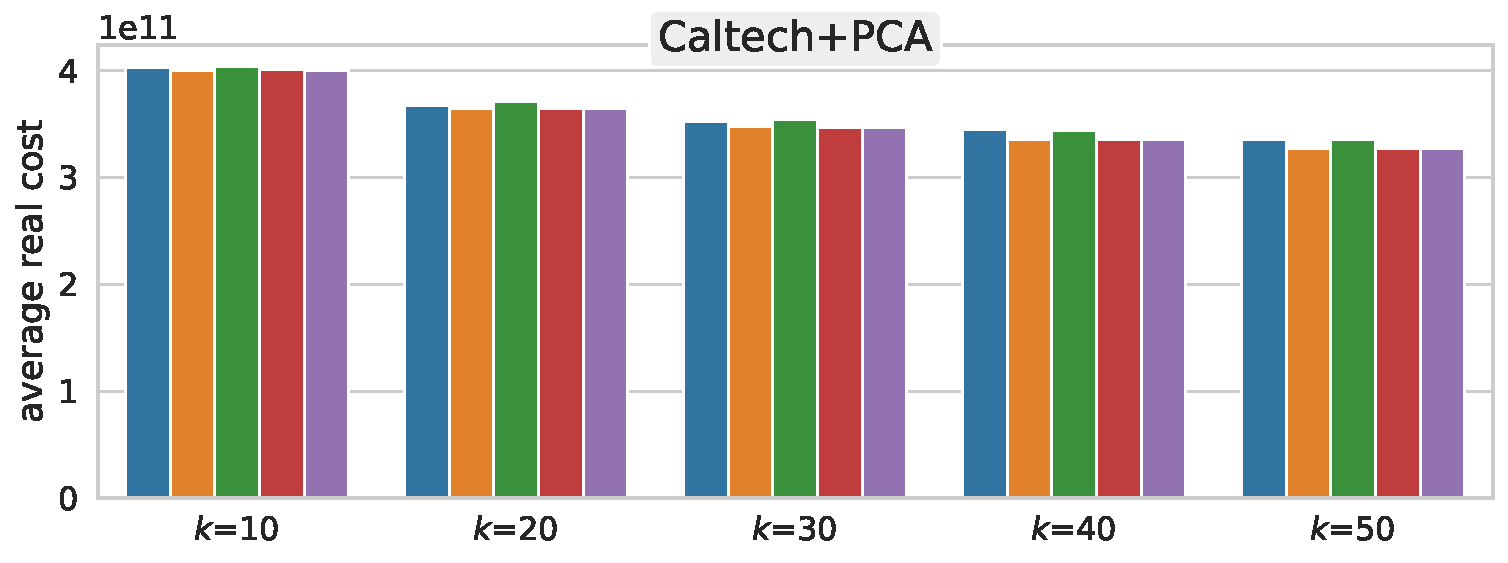
\includegraphics[width=.5\linewidth]{figures/real-costs-Caltech+PCA.pdf}
  }
  \newline\newline
  \subfloat{
    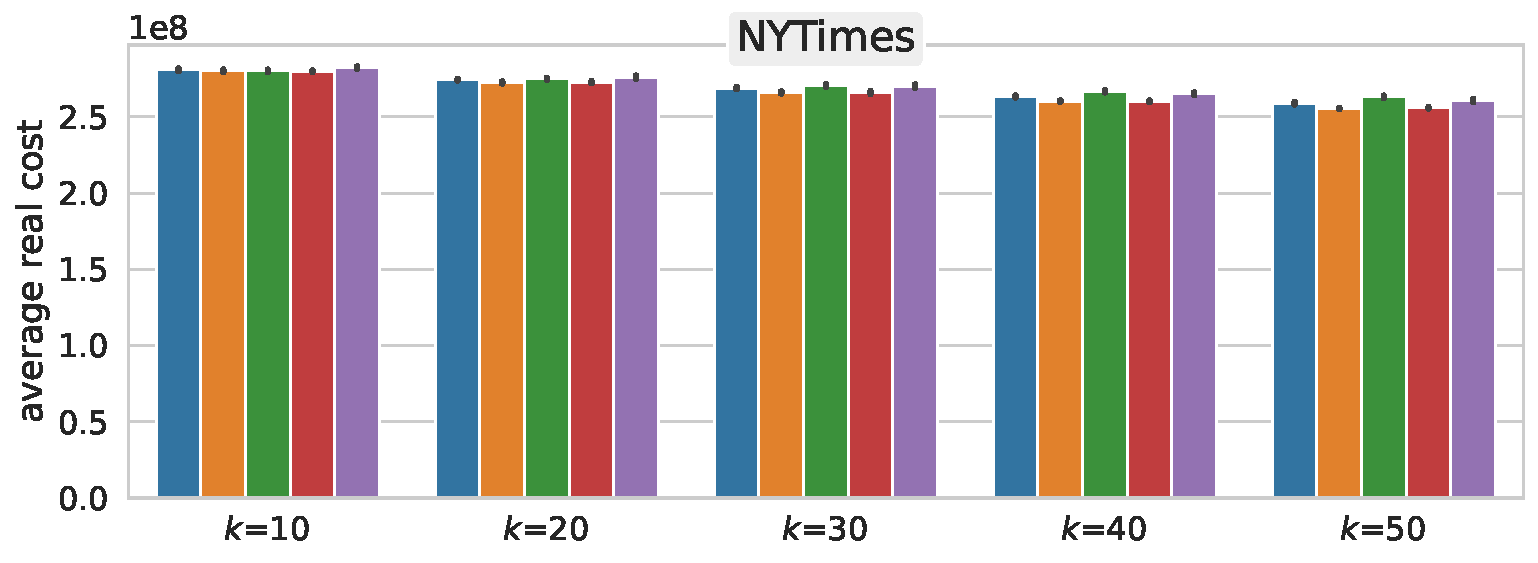
\includegraphics[width=0.5\textwidth]{figures/real-costs-NYTimes.pdf}
  }
  \subfloat{
    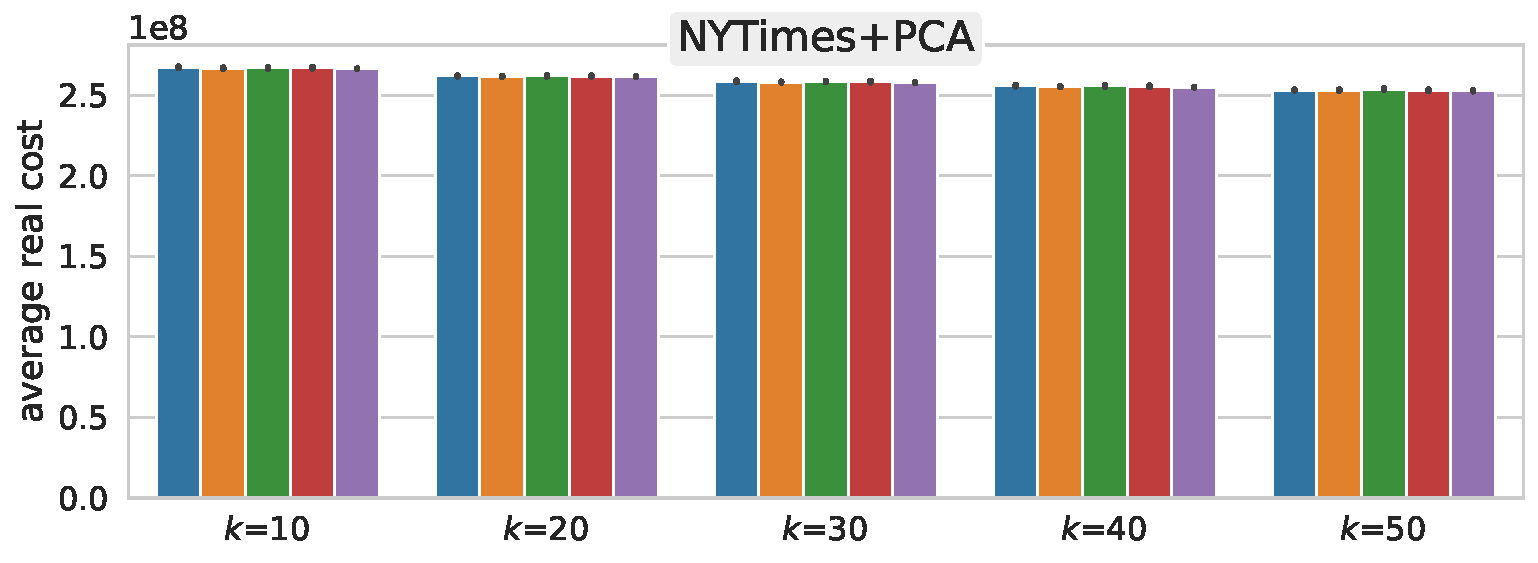
\includegraphics[width=.5\linewidth]{figures/real-costs-NYTimes+PCA.pdf}
  }
  \newline\newline
  \subfloat{
    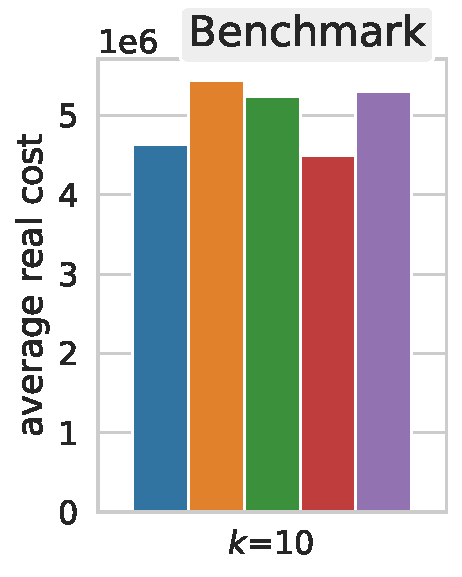
\includegraphics[width=0.15\textwidth]{figures/real-costs-Benchmark-k10.pdf}
    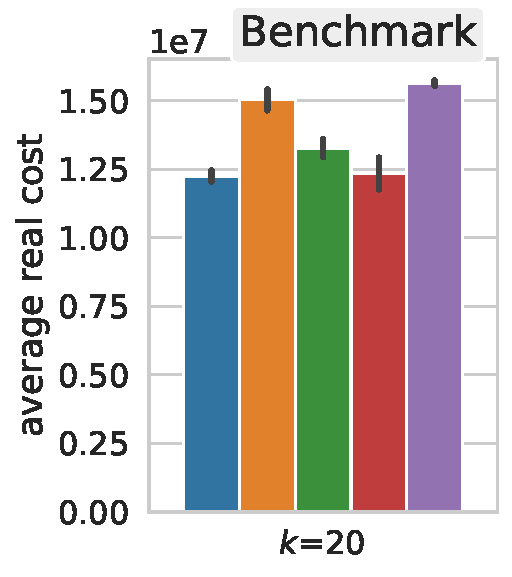
\includegraphics[width=0.165\textwidth]{figures/real-costs-Benchmark-k20.pdf}
    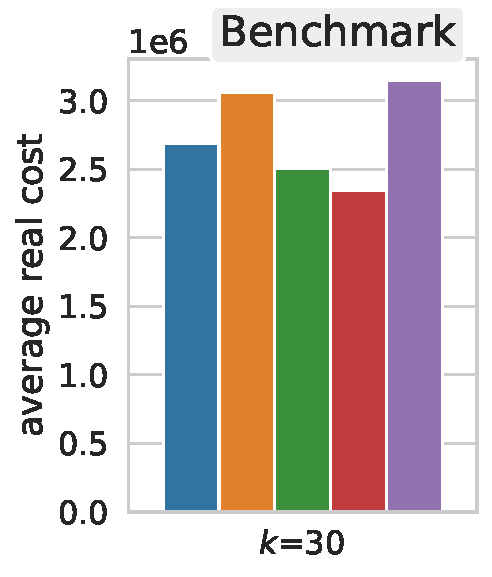
\includegraphics[width=0.16\textwidth]{figures/real-costs-Benchmark-k30.pdf}
    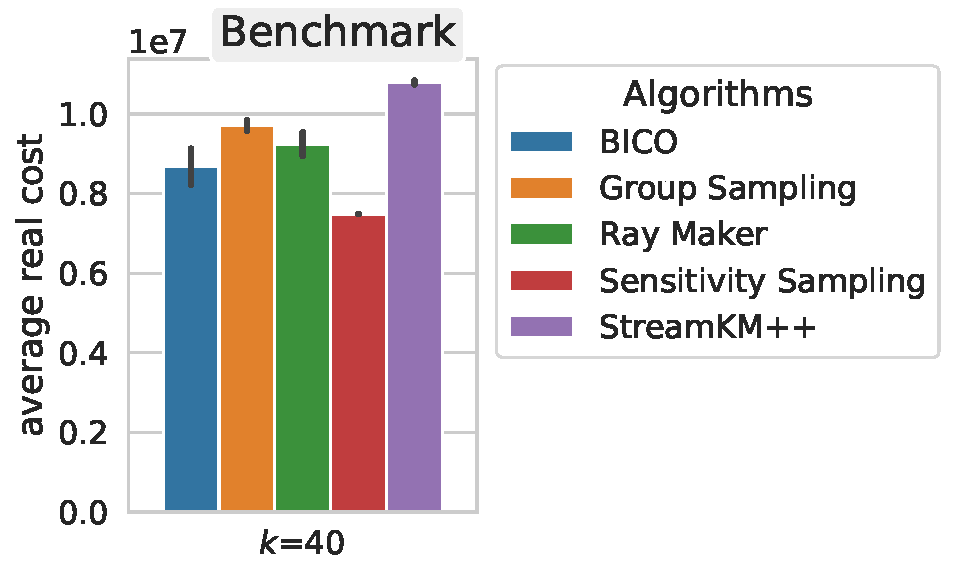
\includegraphics[width=0.31\textwidth]{figures/real-costs-Benchmark-k40.pdf}
  }
  \caption{The average costs of running the evaluated coreset algorithms multiple times on different data sets. In general, the five coreset algorithms are able to compute coresets which result in solutions with comparable costs on the different real-world data sets. The differences in cost is more noticeable on the benchmark instances. Here, Senstivity Sampling is the winner because it seems to be better at capturing the correct ``clusters'' inherent in the benchmark instances.}
  \label{fig:real-costs}
\end{figure*}




